%!TEX root = disclosure_game.tex
%Include the descent into chaos bit
\section{Results}
\label{sec:results}


\subsection{Qualitative Trends}
\label{sub:qt_results}

As shown in figure \ref{fig:honest_signals}, all four decision rules were able to reproduce both qualitative trends towards more disclosure as women experience more appointments \citep{Phillips2007}, and a greater tendency towards underreporting of consumption by heavier drinkers \citep{Alvik2006}.  Trends for all four rules are broadly similar, exhibiting a gradual increase across appointments which subsequently levels off. This levelling can in part be explained by the referral results (figure \ref{fig:referrals}), which show that the majority of drinkers are referred, despite substantial concealment. Referrals continue to occur, in the absence of honest signals, because drinkers are able to achieve a referral by pooling with higher or lower types, dependent on how their initial beliefs are biased. Despite this the results suggest that a minority of drinkers will evade detection altogether, with no notable distinction between heavy and moderate types. Under these parameters, light drinkers always signal honestly and are never referred since there is no perceived advantage in doing so, and the evidence of deceptive signalling is insufficient to outweigh the biased priors of the midwives. 

\begin{figure}[h!]
\begin{adjustbox}{center}\subfloat[Average fraction of population signalling honestly\label{fig:honest_signals}]{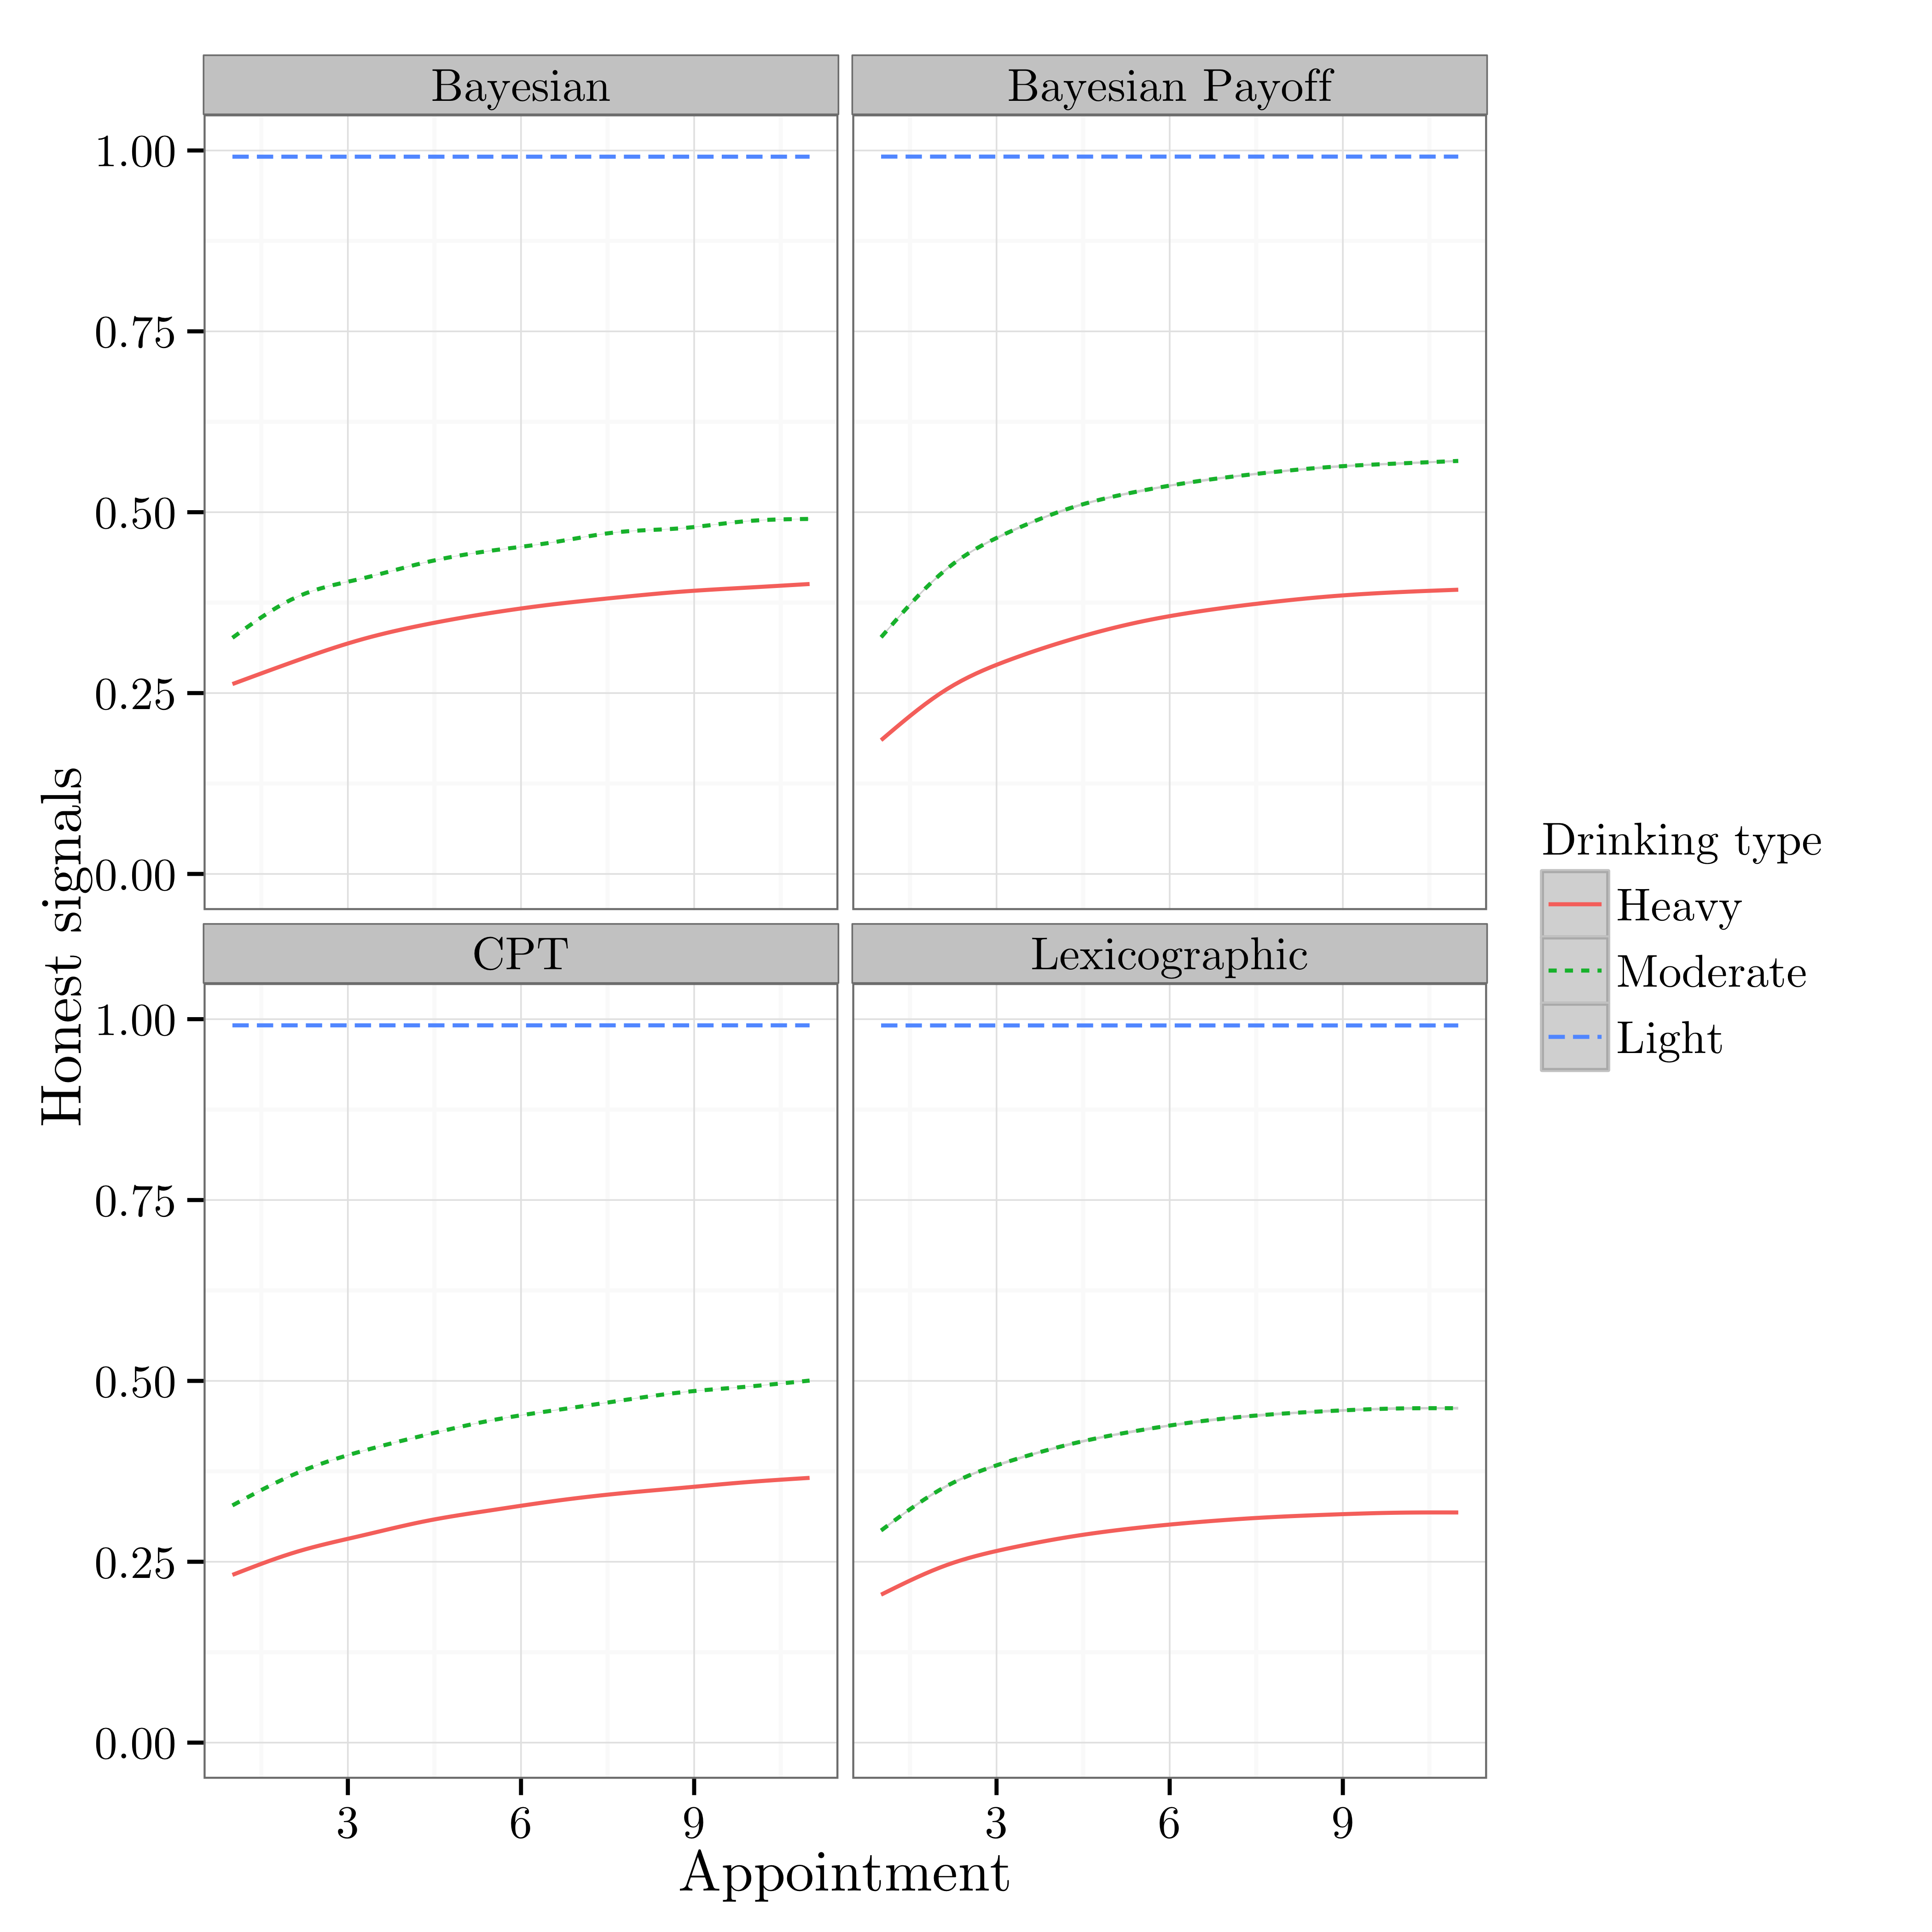
\includegraphics[width=0.43\paperwidth]{figures/honesty_plot.png}

}\subfloat[Average fraction of population referred\label{fig:referrals}]{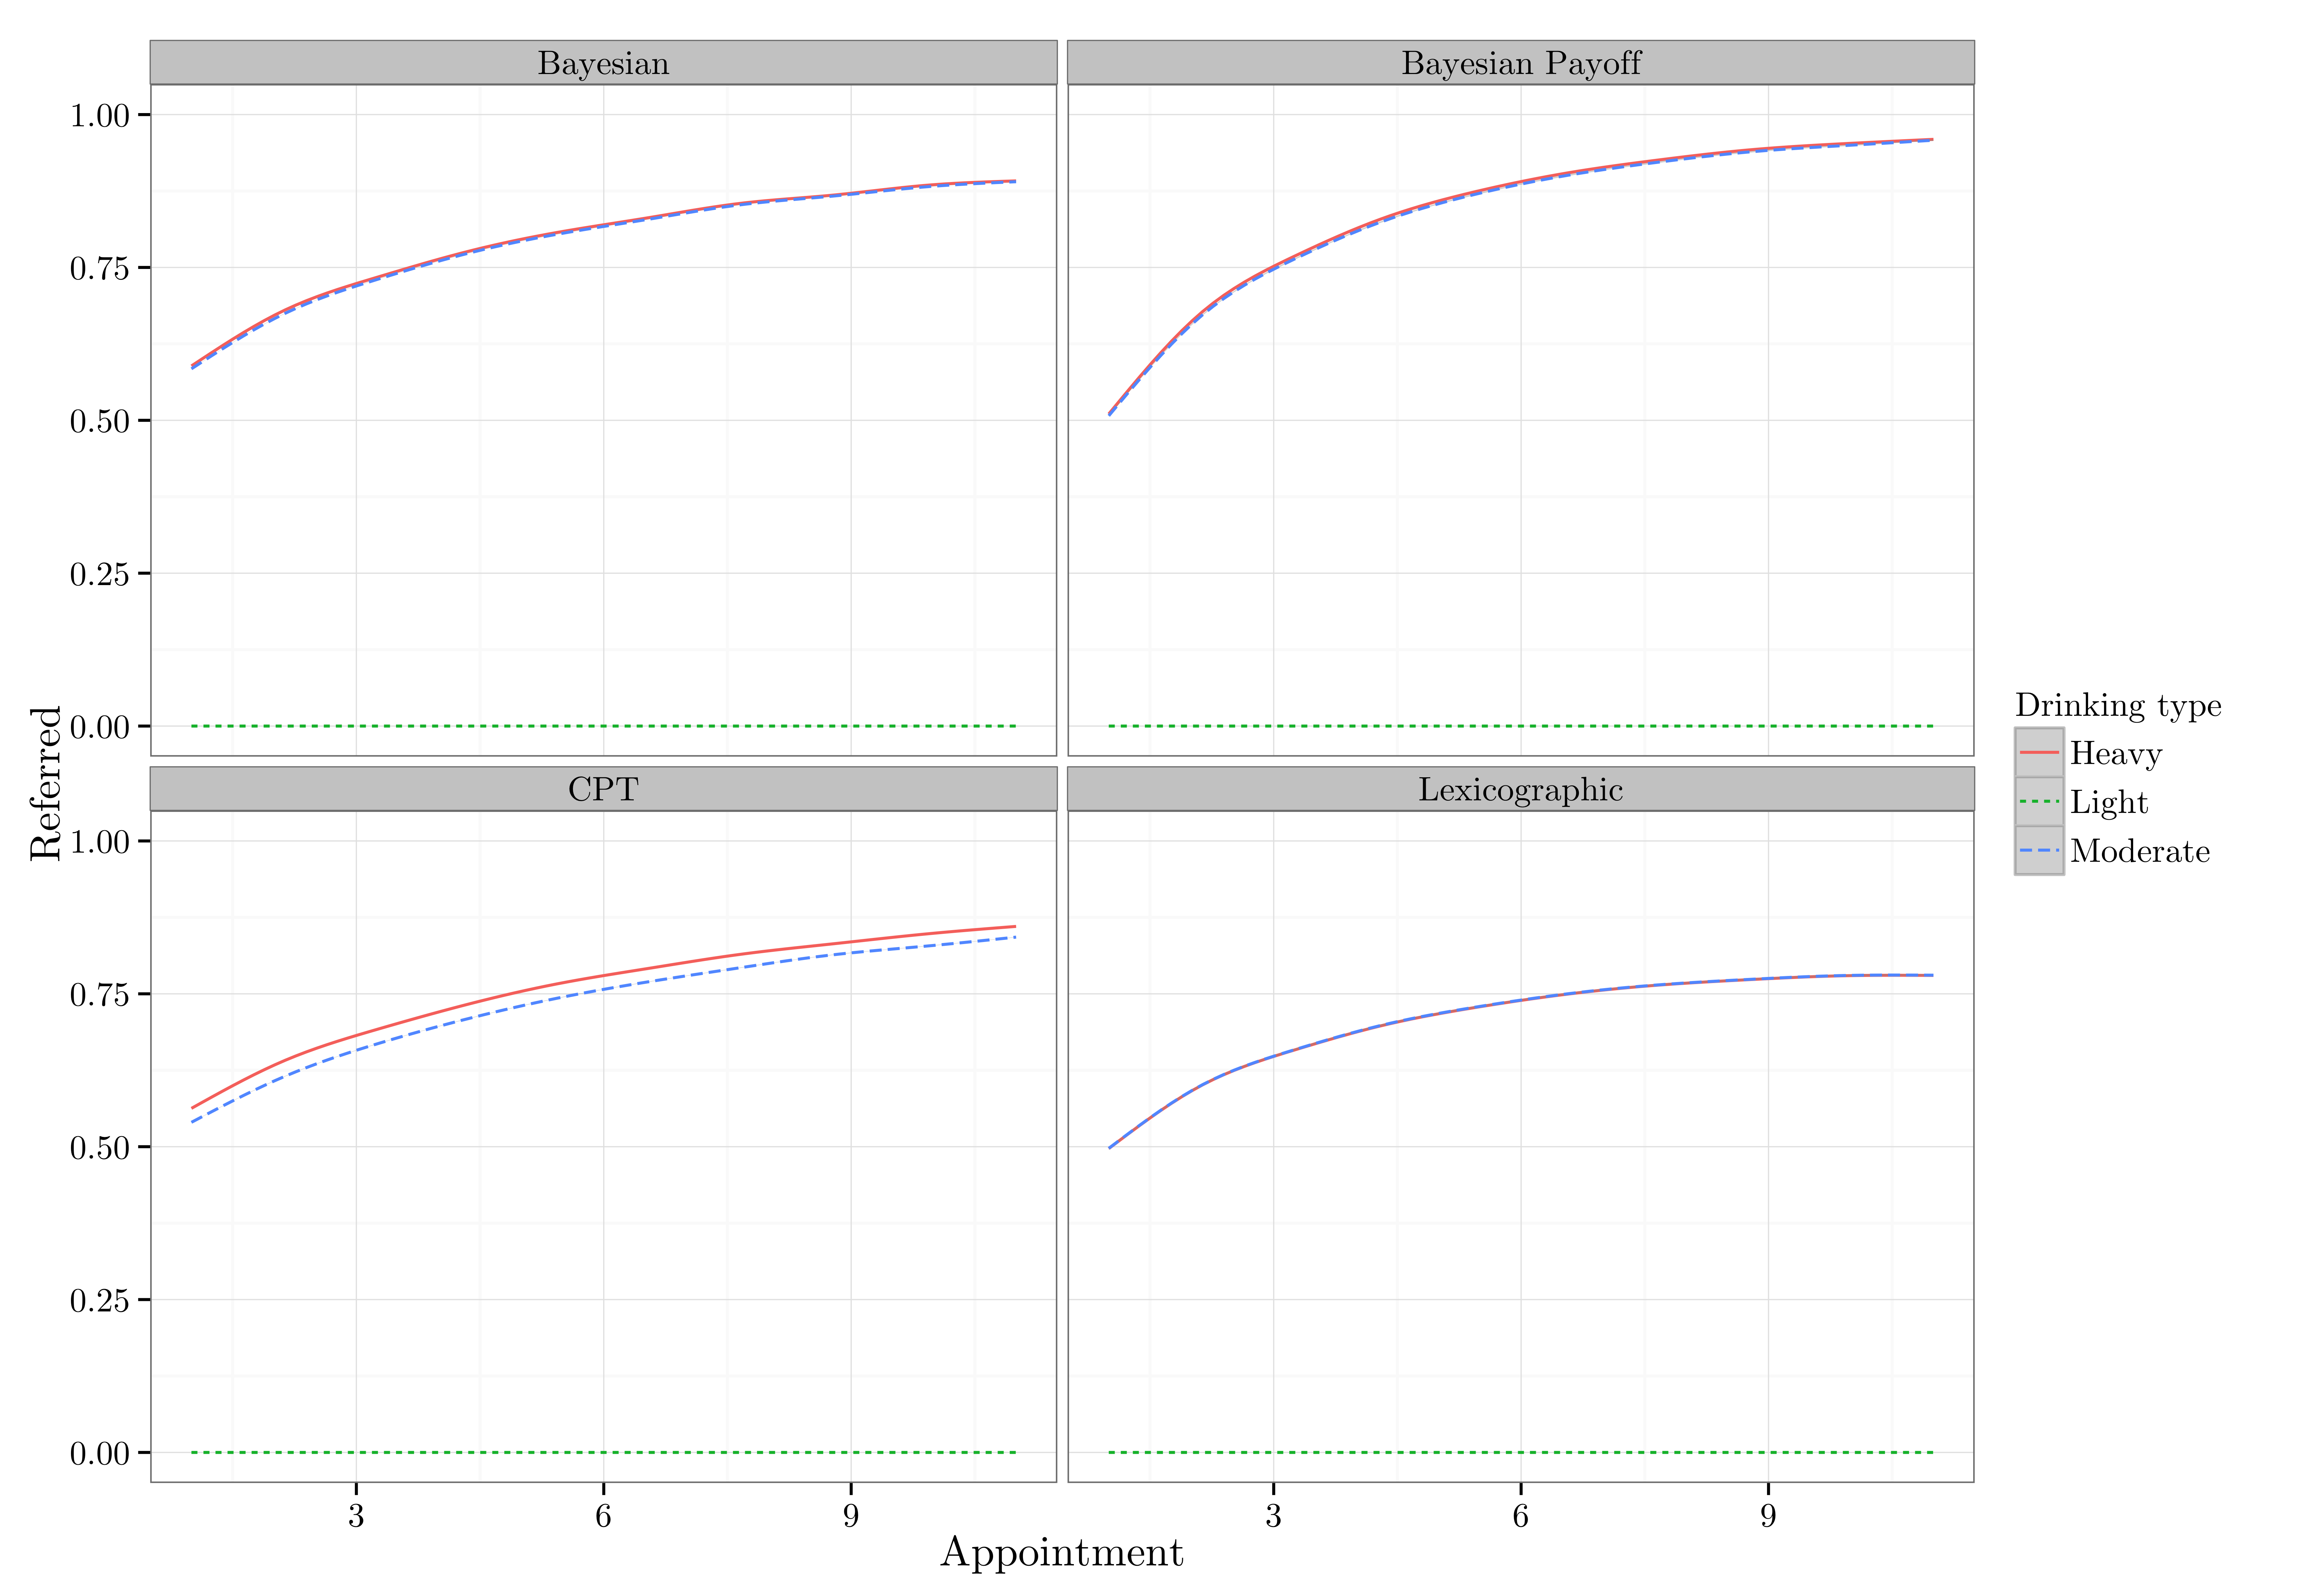
\includegraphics[width=0.43\paperwidth]{figures/ref_plot.png}}\end{adjustbox}
\caption{Qualitative trends after 1000 rounds, mean with 95\% confidence limit over 1000 runs.}
\label{fig:qt_trends}
\end{figure}

\subsection{Information Sharing}
\label{sub:sharing_results}



\subsection{Sensitivity Analysis}
\label{sub:sa_results}

The full results for the sensitivity analysis covering all twelve emulators are available in appendix \ref{}, and in this section we present selected results highlighting......

